\newpage
{\let\clearpage\relax \chapter{正文工具}}

\section{目录}

\section{脚注}

脚注是对正文中词语的补充说明。系统提供的脚注命令如下,序号用于自行设定脚注序号,通常不需要给出。

\begin{latex}{}
\footnote[number]{text}
\end{latex}

例如,为本文作者\footnote{邹思宇,男,\LaTeX 爱好者}添加脚注。

如果要在脚注中输入带反斜杠的字符串,可使用等宽字体命令加字符串命令输入\footnote{\texttt{脚注命令\string\footnote}}。代码如下。如果需要更多的设置,可以调用脚注宏包\qd{footmisc},对脚注命令\verb|\footnote|进行扩展功能。

\begin{latex}{}
\footnote{\texttt{\string\footnote}}
\end{latex}

\section{边注}

\LaTeX 本身提供边注命令:

\begin{latex}{}
\marginpar[左边注]{右边注}
\end{latex}

边注测试\marginpar[这是一个边注]{这是边注啊}。

调用\emph{marginnote}宏包,新定义一个边注。使用\verb|\bz|调用,将会在与段落平齐的地方生成一个边注。例如:

\bz{从这一行开始是用于重新定义边注的代码}

\begin{latex}{}
% 边注和索引,来自重庆大学LaTeX团队
\renewcommand*{\marginfont}{\color{Note}\sffamily\heiti}
\DeclareDocumentCommand{\bz}{s o m}{%
	\IfBooleanTF {#1}
	{%ture
		\IfNoValueTF{#2}{\marginnote[#3]{#3}}{\marginnote[#2]{#3}}
	}{%false
	\IfNoValueTF{#2}{\marginnote[#3]{#3}}{\marginnote[#2]{#3}}
	\index{#3}
}%
}
\end{latex}

\section{参考文献}

中文著作肯定要符合《GB7714-2015信息与文献参考文献著录规则》的要求,我习惯使用biblatex来生成参考文献。在导言区或者自定义的类文件中添加如下1--5行的代码,调用biblatex宏包并指定bib数据库路径\footnote{文中采用的是相对路径,即数据库为我编译的tex文件的同一目录下的Zousiyu.bib文件}和名称。在正文中使用\footnote{一般写在\texttt{\string\end\{document\}}之前}第7行代码打印参考文献。

本书主要参考了刘海洋\cite{刘海洋}和胡伟\cite{胡伟}编写的教程。使用的参考文献样式是胡振震编写的,源码托管在\href{https://github.com/hushidong/biblatex-gb7714-2015}{Github∙hushidong/biblatex-gb7714-2015}上。

\begin{latex}{}
\usepackage[
	backend=biber,%处理方式
	style=gb7714-2015%样式
	]{biblatex}
\addbibresource{Zousiyu.bib}

\printbibliography%打印参考文献
\end{latex}

bib参考文献数据格式如下所示,为分字段显示。各字段可以顾名思义,第一行的“刘海洋”是参考文献标识,你在文中引用参考文献时需要使用此标识。

\begin{latex}{}
@book{刘海洋,
	title={LATEX入门},
	author={刘海洋},
	publisher={电子工业出版社},
	year={2013},
}
\end{latex}

参考文献使用范例,单独列出\cite{刘海洋}\cite{胡伟},一起列出\cite{刘海洋,胡伟}

范例中使用参考文献标识引用参考文献,具体实现如下。

\begin{latex}{}
单独列出\cite{刘海洋}\cite{胡伟}
一起列出\cite{刘海洋,胡伟}
\end{latex}

\section{链接}
这部分内容主要用\qd{hyperref}宏包来实现。

\section{引用功能}\label{tools-ref}
在论文写作中,章节、插图、表格、公式和文本经常要前后调整或增添删减,这些引用的位置难以一次确定,所以不能进行直接编号。\LaTeX 提供很智能的方法来解决这个问题,你不用担心引用的编号问题,只管引用就好了,\LaTeX 系统会帮你编号。

在你的导言区添加如下代码,重新定义自动引用的名字。
\begin{latex}{}
\AtBeginDocument{%
	\def\figureautorefname{图}
	\def\tableautorefname{表}
	\def\partautorefname{卷}
	\def\appendixautorefname{附录}
	\def\equationautorefname{式}
	\def\Itemautorefname{列表}
	\def\chapterautorefname{章}
	\def\sectionautorefname{节}
	\def\subsectionautorefname{小节}
	\def\subsubsectionautorefname{条目}
	\def\paragraphautorefname{自然段}
	\def\Hfootnoteautorefname{脚注}
	\def\AMSautorefname{式}
	\def\theoremautorefname{定理}
	\def\pageautorefname{页}
}
\end{latex}

我们可以使用命令引用一个表格、公式、图片等。如使用如下命令分别引用一张表和一个带编号的公式。引用结果:如\pageref{tools-ref},\autoref{tools-ref}中\autoref{tools-equation},\autoref{tools-tabular},\autoref{tools-figure}所示。




\begin{latex}{}
\ref{tools-equation}
\ref{tools-tabular}
\end{latex}

\begin{equation}\label{tools-equation}
\int arccscx\,dx=xarccscx+ln(x+\sqrt{x^2-1}+C)
\end{equation}

\begin{table}[!ht]
\begin{center}
	\caption{\TeX 家族标识符}
	\label{tools-tabular}
	\begin{tabular}{|C{10mm}|C{10mm}|}
		\hline
		\multicolumn{2}{|c|}{\TeX 家族标识符}\\
		\hline
		\LaTeX & \LaTeXe\\
		\hline
		\TeX & \XeLaTeX\\
		\hline
	\end{tabular}
\end{center}
\end{table}

\begin{figure}[!ht]
	\begin{center}
		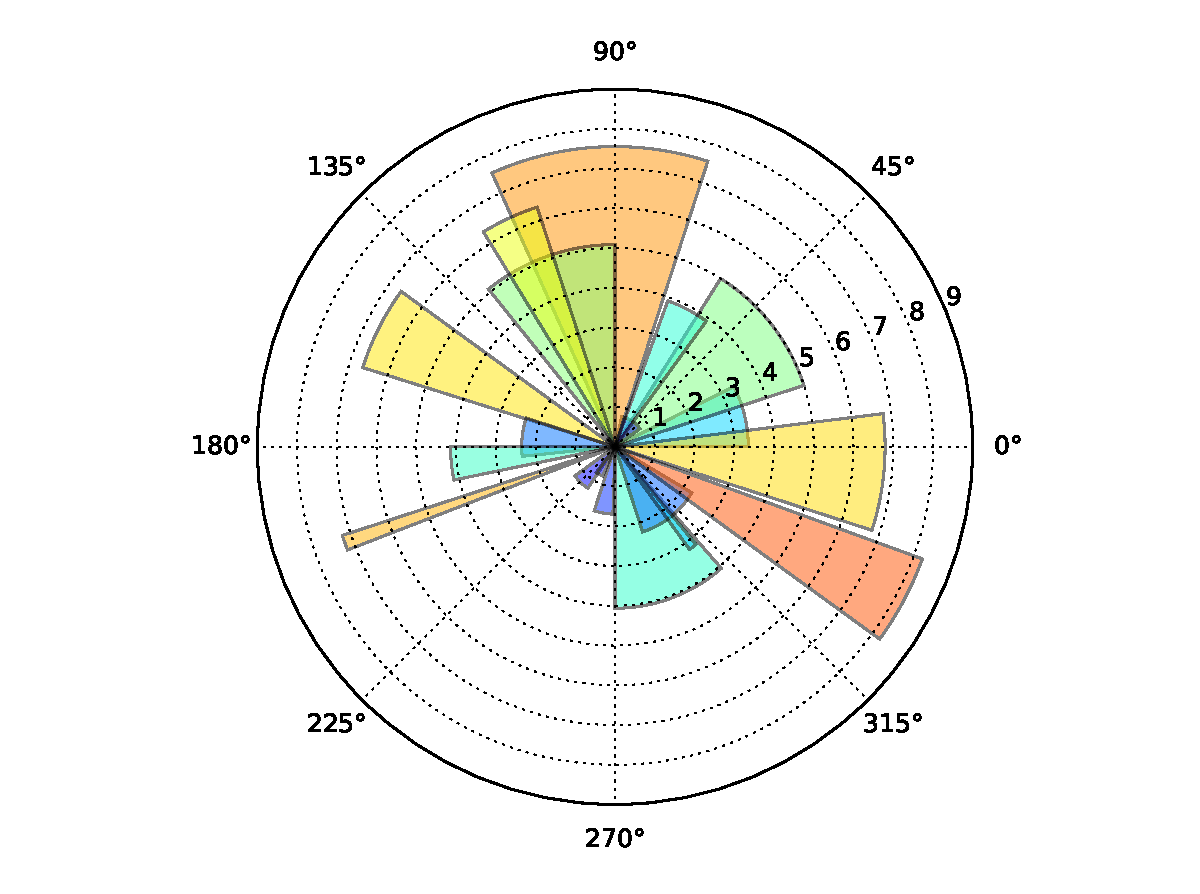
\includegraphics[width=15cm]{tools-figure}
		\caption{Demo of bar plot on a polar axis}
		\label{tools-figure}
	\end{center}
\end{figure}



\section{列表}
\subsection{常规列表}
常规列表环境。

\begin{codeshow}
\begin{itemize}
	\item[记号] 条目1
	\item[-] description1
	\item[*] description2
\end{itemize}
\end{codeshow}

常规列表的条目之间间距较大,可以使用长度赋值命令将条目环境额外的垂直空白设置为0pt,达到与正文间距一致。

\begin{latex}{}
\itemsep=0pt
\parskip=0pt
\end{latex}

\subsection{排序列表}
排序列表的基本形式。

\begin{codeshow}
	\begin{enumerate}
		\item 条目1
		\item 条目2
		\item 条目3
	\end{enumerate}
\end{codeshow}

排序列表可以嵌套,各层条目序号不一,我们可对其序号、标号和前缀进行重新定义,以生成所需要的条目样式。但是重新定义命令使用起来麻烦,排序列表默认命令也复杂,不便记忆,更不便于重定义。

为了方便,我们直接使用\qd{paralist}宏包,我们只需要将标号样式填入方括号中,即可对标号进行重定义。此法在后面说明。

\subsection{解说列表}
示例如下,该类型列表用于对专业术语进行解释。具体设置不做详细说明,因为使用不便,后面有更好的宏包可以对以上所提到的三类列表进行更简便地进行设置。

\begin{codeshow}
	\begin{description}
		\item[APLL] 
		Automatic Phase-Locked Loop
		自动锁相环
		\item[GPS] Global 
		Positioning System 全球定位系统
		\item[SPACETRACK] 
		Space Tracking 空间跟踪
	\end{description}
\end{codeshow}

\subsection{列表宏包}
最常用的列表宏包是\emph{paralist},使用该宏包生成列表,条目与条目之间默认没有额外间距,不需要额外调整。此外,该宏包还提供行内列表,类似于行内公式,非常方便。

\subsubsection{三种常规列表}
\qd{paralist}提供\qd{compactitem,asparaitem,inparaitem}三种常规列表环境。前两种无额外行距,\qd{compactitem}的列表换行也缩进,\qd{asparaitem}换行后无缩进。其中\qd{compactitem}环境可用命令\verb|\pltopsep=12pt|来附加上下额外行距。

在此,我们只看行内列表\qd{inparaitem}一个例子。

\begin{codeshow}
	对于碰撞的物理定义已有许多种,例如:
	\begin{inparaitem}[\S]
		\item 一种以脉冲力相互作用的过程。
		\item 两个质点交换它们动量和能量的持续过程。
	\end{inparaitem}
	我们倾向于第二种说法。
\end{codeshow}

\subsubsection{三种排序列表}
该宏包同样提高三种排序列表环境,\qd{compactenum,asparaenum,inparaenum}。\qd{compactenum}无首行缩进但有换行缩进,\qd{asparaenum}有首行缩进但换行不缩进。

\begin{codeshow}
	对于碰撞的物理定义已有许多种,例如:
	\begin{compactenum}[(1)]
		\item 一种以脉冲力相互作用的过程。
		\item 两个质点交换它们动量和能量的持续过程。
	\end{compactenum}
	我们倾向于第二种说法。
\end{codeshow}

\begin{codeshow}
	对于碰撞的物理定义已有许多种,例如:
	\begin{asparaenum}[(1)]
		\item 一种以脉冲力相互作用的过程。
		\item 两个质点交换它们动量和能量的持续过程。
	\end{asparaenum}
	我们倾向于第二种说法。
\end{codeshow}

宏包提供了一个参数位置,可填入序号和命令来控制排序列表样式。数字必须是\qd{A,a,I,i,1}这几种,否则无法自动排序。如有字符串需要正常输出,可用花括号括起来,如\verb|[{例} 1]|。

\begin{codeshow}
	对于碰撞的物理定义已有许多种,例如:
	\begin{compactenum}[{定义} \itshape (1)]
		\item 一种以脉冲力相互作用的过程。
		\item 两个质点交换它们动量和能量的持续过程。
	\end{compactenum}
	我们倾向于第二种说法。
\end{codeshow}

\subsubsection{三种解说列表环境}
提供\qd{compactdesc,asparadesc,inparadesc}三种解说列表环境,差异见\LaTeXe 完全学习手册列表宏包paralist一节。

\subsubsection{其他特点}
\begin{asparaenum}[(1)]
	\item 调用\emph{paralist}宏包后,系统自带的列表环境也可以使用可选参数来修改条目标志和样式。
	\item 支持交叉引用。
	\item 常规列表和排序列表可以相互嵌套。
\end{asparaenum}

\begin{codeshow}
	调用\emph{paralist}宏包后,系统自带的列表环境的标记更改示例。
	\begin{enumerate}[(1)]
		\itemsep=0pt
		\parskip=0pt
		\item 条目1
		\item 条目2
		\item 条目3
		\end{enumerate}
\end{codeshow}

\section{附录}

\section{代码环境}

首先载入\emph{listings}宏包,定义基础代码环境,我取名为\emph{CodeBase},这个基础代码环境定义的样式能被后续的代码环境调用,免去重复设置。也正是因为基础代码环境的通用性,所以这里只适合定义在所有代码环境中都适用的样式,如字体、各种边距、换行和标识等。

\begin{latex}{}
\lstdefinestyle{CodeBase}
{
	basicstyle=\small\ttfamily,
	frame=l,
	aboveskip=0pt,%上边距
	belowskip=0pt,%下边距
	lineskip=0pt,
	tabsize=4,%设置tab空格数
	showtabs=false,%Tab
	showspaces=false,%空格标识
	showstringspaces=false,
	numbers=left,
	numbersep=5pt,%行号与代码距离
	numberstyle=\small\ttfamily,
	rulecolor=\color{cyan},
	boxpos=c,
	xleftmargin=1em,%左边距
	xrightmargin=0pt,
	breaklines=true,%自动换行
	breakindent=0pt,%换行后缩进为0
	extendedchars=false,%解决代码跨页时,章节标题,页眉等汉字不显示的问题
	framesep=3pt,
	rulesep=2pt,
	framerule=1pt,
	%代码颜色设置
	backgroundcolor=\color{gray!5},
	stringstyle=\color{green!40!black!100},
	keywordstyle=\bfseries\color[RGB]{0,0,255},
	commentstyle=\slshape\color{black!60},
}
\end{latex}

接下来,我们就可以用这个基本样式来定义一个专用于\LaTeX 代码书写的样式和相应的环境。

\begin{latex}{}
%LaTeX代码环境用
\lstdefinestyle{LaTeX}
{
	style=CodeBase,
	language=[LaTeX]TeX,
	classoffset=0,
	morekeywords={addplot, begin, end},
}

%定义latex代码专用环境
\lstnewenvironment{latex}[1]{\lstset{style=LaTeX}}{}
\end{latex}

最后,直接在正文中使用新定义的环境\emph{latex}框住所需要展示的代码即可。

上面定义了一个\LaTeX 专用的代码环境,实际使用肯定不只\LaTeX 代码需要展示,还有诸如\emph{Python},\emph{MATLAB}等大量其他代码需要展示。这里我们在定义一个用于展示\emph{MATLAB}代码的环境,同样也是从基础样式\emph{CodeBase}进行衍生,只需要几条简单的命令即可。

\begin{latex}{}
%matlab代码展示
\lstdefinestyle{Matlab}{
	style=CodeBase,
	language=Matlab
}

%定义Matlab代码专用环境
\lstnewenvironment{Matlab}[1]{\lstset{style=Matlab}}{}
\end{latex}

MATLAB代码高亮测试。

\begin{Matlab}{}
t=0:pi/10:2*pi;
[X,Y,Z]=cylinder(4*cos(t));
subplot(1,2,1);mesh(X);title('X');
subplot(1,2,2);mesh(Y);title('Y');
\end{Matlab}

从\emph{CodeBase}定义的新样式X,其设置可以覆盖\emph{CodeBase}中的设置,如下面这段\emph{Python}代码高亮测试中,我们在代码中定义了一句\verb|keywordstyle=\slshape\color[RGB]{0,0,255},|,让\emph{Python}代码中的关键词变为斜体,其他代码环境不受影响。

\begin{latex}{}
\lstdefinestyle{python}{
	style=CodeBase,
	keywordstyle=\slshape\color[RGB]{0,0,255},%%%%%%%就是这句
	language=Python,
	morekeywords={def},
}
\lstnewenvironment{python}[1]{\lstset{style=python}}{}
\end{latex}

\emph{Python}代码展示。

\begin{python}{}
def ffmpeg_concat_av(files, output, ext):
	print('Merging video parts... ', end="", flush=True)
	params = [FFMPEG] + LOGLEVEL
	for file in files:
		if os.path.isfile(file): params.extend(['-i', file])
	params.extend(['-c:v', 'copy'])
	if ext == 'mp4':
		params.extend(['-c:a', 'aac'])
	elif ext == 'webm':
		params.extend(['-c:a', 'vorbis'])
	params.extend(['-strict', 'experimental'])
	params.append(output)
	return subprocess.call(params)
\end{python}

\emph{listings}宏包识别的代码关键词肯定是有限的,但好在它提供一个参数可以扩充关键词。比如我们为\emph{c++}语言添加更多的关键词,只需要在设置里面写下如下代码。关键词想要多少都行,依据实际情况补充。

\begin{latex}{}
\lstset{
	morekeywords={alignas,continute,friend,register,true,alignof,decltype,goto,reinterpret_cast,try,asm,defult,if,return,typedef,auto,delete,inline,short,typeid,bool,do,int,signed,typename,break,double,long,sizeof,union,case,dynamic_cast,mutable,static,unsigned,catch,else,namespace,static_assert,using,char,enum,new,static_cast,virtual,char16_t,char32_t,explict,noexcept,struct,void,export,nullptr,switch,volatile,class,extern,operator,template,wchar_t,const,false,private,this,while,constexpr,float,protected,thread_local,const_cast,for,public,throw,std}
},
\end{latex}


